\documentclass{article}
\usepackage[utf8]{inputenc}
\usepackage{listings}
\usepackage{graphicx}
\usepackage{float}

\setlength{\parindent}{0pt}
\lstset{
    basicstyle=\ttfamily\footnotesize,
    frame=single,
    xleftmargin=4pt,
    xrightmargin=4pt,
}

\title{Lab Report: Particle Argon Peripherals}
\author{Lue Xiong}

\begin{document}

\maketitle
\newpage
\obeylines

\section{Introduction}
The focus of the lab is to gain a basic understanding of what analog and digital signals are and how they relate to one another. For this lab, we are using resistors on an analog pin to manipulate the analog values, capture and convert them into digital values. Calculations will be done beforehand to predict the analog-to-digital (ADC) values with a margin of error percentage. The predicted ADC outputs will be compared with the actual readings coming from the Particle Argon. The idea is to get familiar by grounding our understanding with real-world instances.

\section{Problem Statement}
The lab can be summarized down to five main different parts, which include:

\begin{itemize}
\item RGB LED -- Utilize Particle Argon's pulse-width modulation capability on pins \textit{D2}, \textit{D3}, and \textit{D4}
\item Piezzo Buzzer -- Modify the code to play the same sequence as the “two-bits.mp4”
\item Switches --
\item Servo --
\item Analog Temperature Sensor -- 
\end{itemize}

\section{Process}
\subsection{Part One: RGB LED}
\begin{figure}[H]
\center
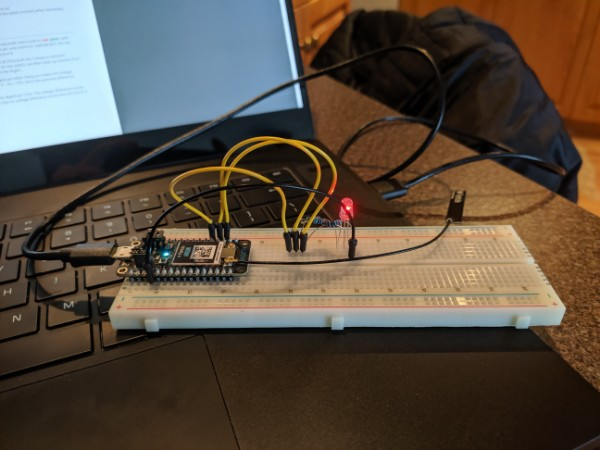
\includegraphics[width=\textwidth]{images/fade.jpeg}
\caption{Particle Argon RGB LED}
\label{fig:fade}
\end{figure}

The code below shows how to create the fade effect on the RGB LED by using a function called \textbf{fade()}. The function starts with a loop that increments \textit{brightness} by 1 from 0 to 255 with 10 millisecond delays in between. Upon reaching \textit{brightness} value 255, another loop will run and decrement by 1 from 255 to 0 with 10 millisecond delays in between. It is in practice, a rather slow fade but it works nonetheless. Figure~\ref{fig:fade} is a photo of the components composition on the breadboard.\\

\lstinputlisting[language=C]{../archive/rgb-led.ino}

\subsection{Part Two: Piezzo Buzzer}
\begin{figure}[H]
\center
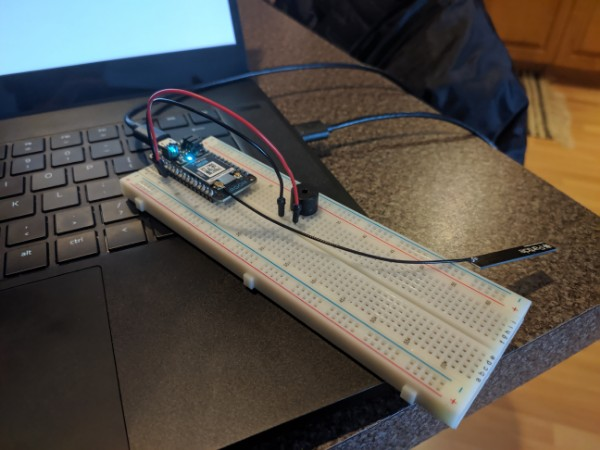
\includegraphics[width=\textwidth]{images/buzzer.jpeg}
\caption{Particle Argon Piezzo Buzzer}
\label{fig:buzzer}
\end{figure}

The code below shows how to create the two-bits sound on the piezzo buzzer by using a function called \textbf{twoBitsBuzz()}. The function sends currents of multiple levels to the piezzo buzzer at arbritrary times in attempt to mimic the "two-bits.mp4" tune. Figure~\ref{fig:fade} is a photo of the components composition on the breadboard.\\

\lstinputlisting[language=C]{../archive/piezzo-buzzer.ino}

\subsection{Part Three: Switches}
\begin{figure}[H]
\center
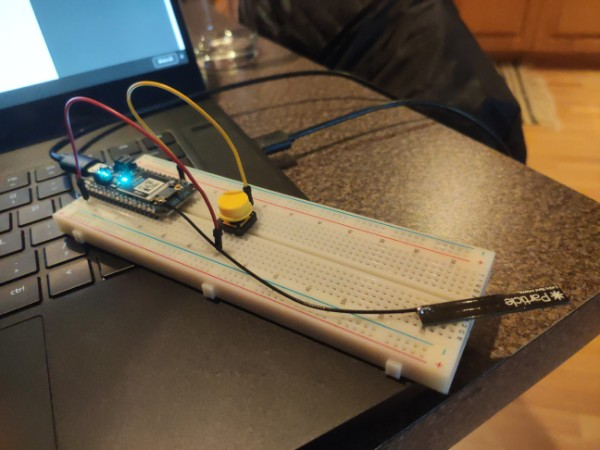
\includegraphics[width=\textwidth]{images/switches.jpeg}
\caption{Particle Argon Switches}
\label{fig:switches}
\end{figure}

When the momentary switch is depressed, it engages metal to metal contact which creates a circuit for currents to run through. When it is released from being depressed, the circuit is broken. In this context, assuming the momentary switch is depressed, 3.3 volts will flow from the \textbf{3V3} pin to the \textbf{D2} pin and keep looping as such. Essentially this is what happens when \textbf{mom = 1}.\\

\begin{figure}[H]
\center
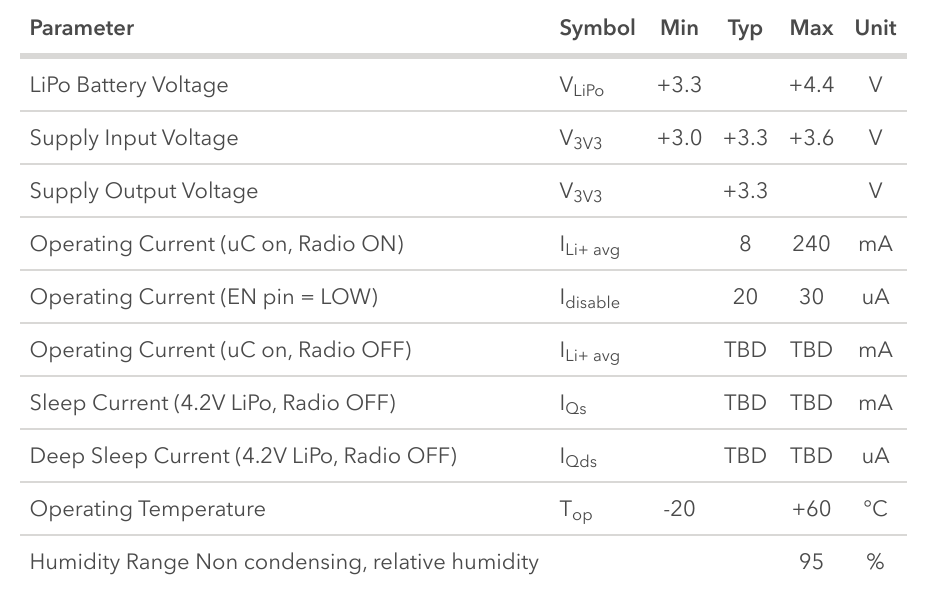
\includegraphics[width=\textwidth]{images/operating-conditions.png}
\caption{Particle Argon Operating Conditions}
\label{fig:operating}
\end{figure}

As shown on Figure~\ref{fig:operating} -- more specifically the \textbf{Supply Input Voltage} parameter -- the minimum voltage stated is 3.0 volts for inputs like momentary switches. Interestingly enough, the maximum voltage is 3.6 volts, which means that there is a +/- 0.3 volt difference from the typical 3.3 volt.\\

\lstinputlisting[language=C]{../archive/switches.ino}\ \\

The code above produces the outputs on the serial monitor in Figure~\ref{fig:mom}. The \textbf{mom = 0} state means that there is no physical connection between the \textbf{3V3} and \textbf{D2} pin. The \textbf{mom = 1} means that the momentary switch is depressed to create a physical connection between \textbf{3V3} and \textbf{D2} pin.

\begin{figure}[H]
\center
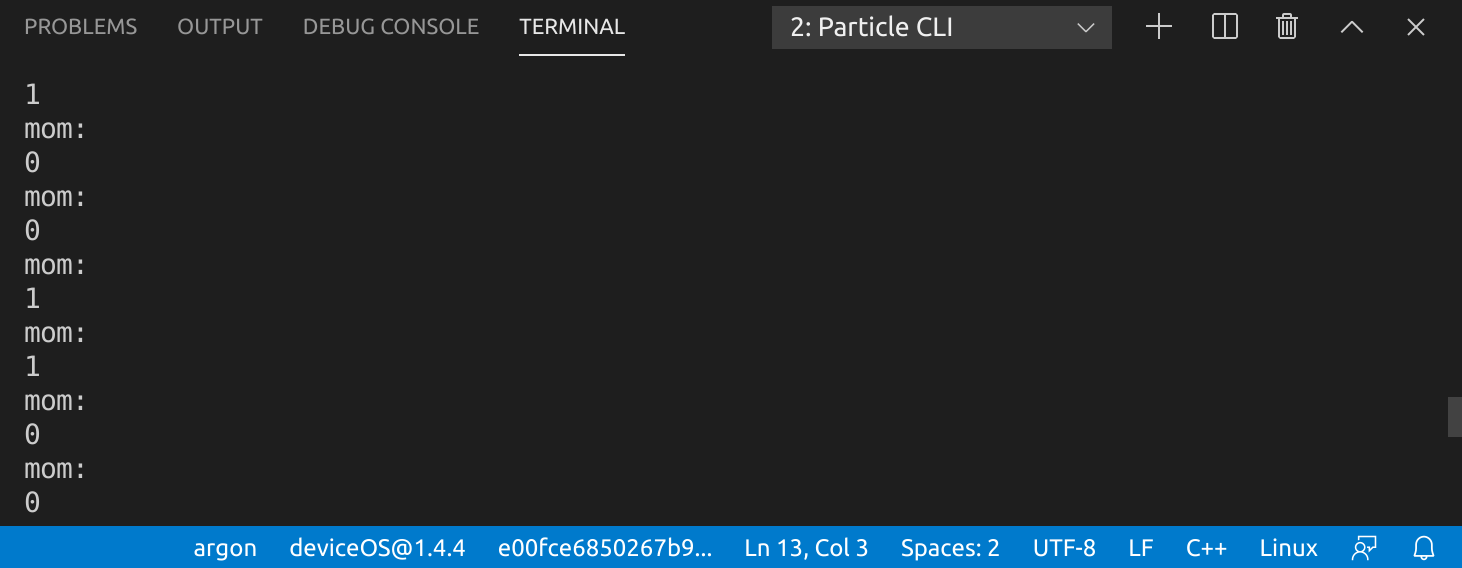
\includegraphics[width=\textwidth]{images/mom.png}
\caption{Particle Argon Switches}
\label{fig:mom}
\end{figure}

\subsection{Part Four: Servo}
\begin{figure}[H]
\center
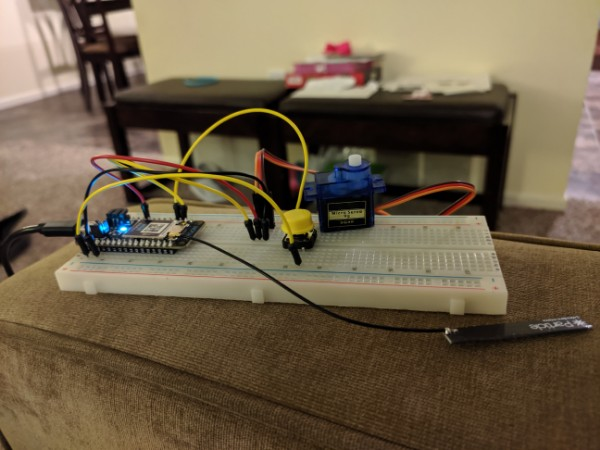
\includegraphics[width=\textwidth]{images/servo.jpeg}
\caption{Particle Argon Servo}
\label{fig:servo}
\end{figure}

\lstinputlisting[language=C]{../archive/servo.ino}

\subsection{Part Five: Analog Temperature Sensor}


\section{Discussion of Results}


\section{Conclusion}


\end{document}